%!TEX root = main.tex

\section{Linear Programing: The simplex method}\index{Simplex method}\index{Linear programming}

A general linear program $(LP)$ is usually expressed in the following standard form:
\begin{equation*}
(LP): \begin{cases}
\displaystyle{\max_{\x \in \field{R}^d} \langle \boldsymbol{c}, \x \rangle} \\
\langle \boldsymbol{a}_j, \x \rangle = b_j &(1 \leq k \leq \ell) \\
x_k \geq 0 &(1 \leq k \leq d) 
\end{cases}
\end{equation*}
for a given $\boldsymbol{c}=[c_1, \dotsc, c_d], \boldsymbol{a}_k = [a_{k1}, \dots, a_{kd} ] \in \field{R}^d$, $b_k \in \field{R}$ for $1 \leq k \leq \ell$.  We accomplish this by performing the following operations, where necessary:
\begin{description}
	\item[Objective function] If the original program requests $\min f(\x)$, convert it to $\max \big( -f(\x) \big)$.
	\item [Slack variables] If the original program contains an inequality constraint of the form $\langle \boldsymbol{a}, \x \rangle \leq b$ with $\boldsymbol{a} = [a_1, \dotsc, a_d]$, convert it to an equality constraint by adding a non-negative \emph{slack variable}\index{Simplex method!slack variable} $s$. The resulting constraint is 
	\begin{equation*}
	a_1 x_1 + \dotsb + a_d x_d + s = b, \quad s \geq 0.
	\end{equation*}
	\item [Surplus variables] If the original program contains an inequality constraint of the form $\langle \boldsymbol{a}, \x \rangle \geq b$, convert it to an equality constraint by subtracting a non-negative \emph{surplus variable}\index{Simplex method!surplus variable} $s$.  The resulting constraint is
	\begin{equation*}
	a_1 x_1 + \dotsb + a_d x_d - s = b, \quad s \geq 0.
	\end{equation*}
	\item[Unrestricted variables in sign]\index{Simplex method!Unrestricted variables in sign} If some variable $x_k$ is unrestricted in sign, replace it every where in the formulation by $x_k^+ - x_k^-$, where $x_k^+ \geq 0$ and $x_k^- \geq 0$.
\end{description}

\separator 

Once in standard form, we usually represent a linear program by its corresponding \emph{tableau}:\index{Simplex method!tableau}\index{tableau}
\begin{equation*}
\begin{bmatrix} 1 & -\boldsymbol{c} & 0 \\ \transpose{\boldsymbol{0}} & \boldsymbol{A} & \transpose{\boldsymbol{b}} \end{bmatrix},
\end{equation*}
where
\begin{equation*}
\boldsymbol{A} = \begin{bmatrix} a_{11} & \dotsb & a_{1d} \\ \vdots & \ddots & \vdots \\ a_{\ell 1} & \dotsb & a_{\ell d} \end{bmatrix}
\end{equation*}
and $\boldsymbol{b} = [b_1, \dotsc, b_\ell]$.

\begin{example}\label{example:FirstLinearProgram}
Consider the linear program $(LP)$ given by the no-standard formulation
\begin{equation*}
(LP): \begin{cases}
\displaystyle{\min_{(x,y,z) \in \field{R}^3} \big( 3y-2x \big)} \\
x - 3y + 2z \leq 3, \\
2y-x \geq 2, \\
y \geq 0, z \geq 0 \\
\end{cases}
\end{equation*}
We can easily convert the objective function to a maximum, and the first two inequality constraints into equality constraints by introducing a slack variable $s_1 \geq 0$ and a surplus variable $s_2 \geq 0$.  Notice that the variable $x$ is unrestricted in sign.  We convert it into two non-negative variables $x^+ - x^-$:
\begin{equation*}
\left\{
\begin{matrix}
\displaystyle{\max_{(x,y,z) \in \field{R}^3}} & \big( 2x^+ & -2x^- &-3y \big) \\
& x^+ & -x_- & -3y & +2z & +s_1 & & = 3, \\
& -x^+ & +x^- & +2y & & &-s_2 &= 2, \\
&x^+ \geq 0, &x^- \geq 0, &y \geq 0, &z \geq 0, &s_1 \geq 0, &s_2 \geq 0 
\end{matrix}
\right.
\end{equation*}
The corresponding tableau is as follows:
\begin{equation*}
\begin{bmatrix}
1 & -2 & 2  & 3  & 0 & 0 & 0  & 0\\
0 & 1  & -1 & -3 & 2 & 1 & 0  & 3 \\
0 & -1 &  1 & 2  & 0 & 0 & -1 & 2
\end{bmatrix}
\end{equation*}
\end{example}

\separator

The \emph{Simplex method} to find the optimal solution of a linear program in standard form is based on the following two rules:
\begin{description}
	\item[Rule 1] If all variables have a nonnegative coefficient on the first row, the current basic solution (the last column) is optimal.  Otherwise, pick a variable $x_k$ with a negative coefficient $(-c_k)$ in the first row---the \emph{entering variable}\index{Simplex method!entering variable}---and \emph{pivot} it with another row.

	\item[Rule 2] The selection of row to perform the pivot for the entering variable $x_k$ is performed by choosing among the rows $j$ for which $a_{jk} > 0$, the one with the minimum ratio $b_j/a_{jk}$.
\end{description}

\begin{example}
Let's illustrate this process with the following linear program
\begin{equation*}
(LP): \begin{cases}
\displaystyle{\max_{(x,y) \in \field{R}^2} \big( x+y \big)} \\
2x+y \leq 4 \\
x+2y \leq 3 \\
x \geq 0, y \geq 0
\end{cases}
\end{equation*}
We start by converting to standard.  For ease of computations below, we first rename $x=x_1$ and $y=x_2$.  We introduce the slack variables $x_3$ and $x_4$ as they are needed.  We finish the preparation step by finding the tableau of this program.
\begin{equation*}
(LP): \left\{
\begin{matrix}
\displaystyle{\max_{(x,y) \in \field{R}^2}} &\big( x_1   & +x_2 \big) \\
                                            &2x_1        & +x_2        & +x_3        &          &= 4 \\
                                            &x_1         & +2x_2       &             & +x_4     &= 3 \\
                                            &x_1 \geq 0, & x_2 \geq 0, & x_3 \geq 0, &x_4 \geq 0
\end{matrix}
\right.
\end{equation*}
\begin{equation*}
\begin{bmatrix}
1 & \boldsymbol{-1}  & -1  & 0   & 0   & 0\\
0 & 2                & 1   & 1   & 0   & 4 \\
0 & 1                & 2   & 0   & 1   & 3 \\ \hline
z & x_1              & x_2 & x_3 & x_4 
\end{bmatrix}
\end{equation*}
At this stage, we have the following initial situation:
\begin{equation*}
z=0 \qquad \underbrace{x_3=4, \quad x_4=3}_{\text{basic solutions}} \qquad \underbrace{x_1=x_2=0}_{\text{non-basic solutions}}
\end{equation*}
The first entering variable is $x_1$.  We have two choices to pivot.  Rule 2 indicates that we must use the second row, since for this row, we have the ratio $4/2 = 2$, while the third row offers a bigger ratio: $3/1=3$.
\begin{equation*}
\begin{bmatrix}
1 & -1  & -1  & 0   & 0   & 0\\
0 & 1   & 1/2 & 1/2 & 0   & 2 \\
0 & 1   & 2   & 0   & 1   & 3 \\ \hline
z & x_1 & x_2 & x_3 & x_4 
\end{bmatrix} \to 
\begin{bmatrix}
1 & 0   & \boldsymbol{-1/2} & 1/2  & 0   & 2\\
0 & 1   & 1/2               & 1/2  & 0   & 2 \\
0 & 0   & 3/2               & -1/2 & 1   & 1 \\ \hline
z & x_1 & x_2               & x_3 & x_4 
\end{bmatrix}
\end{equation*}
At this stage, we have the following situation:
\begin{equation*}
z = 2 \qquad \underbrace{x_1 = 2, \quad x_4 =1}_{\text{basic solution}} \qquad \underbrace{x_2=x_3=0}_{\text{non-basic solution}}
\end{equation*}
The second entering variable is $x_2$.  We again have two choices to pivot.  Rule 2 indicates that we must use the third row, since for this row the ratio is $1/(3/2)=2/3$.  For the second row, the ratio is larger: $2/(1/2)=4$.
\begin{equation*}
\begin{bmatrix}
1 & 0   & -1/2 & 1/2  & 0   & 2\\
0 & 1   & 1/2  & 1/2  & 0   & 2 \\
0 & 0   & 1    & -1/3 & 2/3 & 2/3 \\ \hline
z & x_1 & x_2  & x_3  & x_4 
\end{bmatrix} \to 
\begin{bmatrix}
1 & 0   & 0   & 1/3  & 1/3  & 7/3 \\
0 & 1   & 0   & 2/3  & -1/3 & 5/3 \\
0 & 0   & 1   & -1/3 & 2/3  & 2/3 \\ \hline
z & x_1 & x_2 & x_3  & x_4 
\end{bmatrix}
\end{equation*}
There are no more negative coefficients on the first row.  This leads to an solution of the tableau given by $z=7/3$, $x_1=5/3$. $x_2=2/3$, $x_3=x_4=0$.  The global maximum of the function $f(x,y)=x+y$ on the set $S = \{ (x,y) \in \field{R}^2: x\geq 0, y \geq 0, 2x+y \leq 4, x+2y \leq 3 \}$ is attained at the point $(5/3, 2/3)$.  The corresponding maximum value is thus $7/3$.  An illustration of the three steps carried in these computations can be observed in Figure \ref{figure:simplexmethod}.
\begin{figure}[ht!]
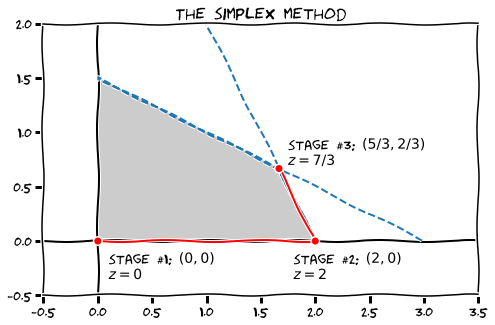
\includegraphics[width=0.75\linewidth]{images/simplex.png}
\caption{Illustration of the simplex method for Example \ref{example:FirstLinearProgram}}
\label{figure:simplexmethod}
\end{figure}
\end{example}

\begin{example}
What happens if the program does not have a unique solution?  Can the simplex method offer this information? Consider for $f(x,y)=x+\tfrac{1}{2}y$ the program
\begin{equation*}
(LP): \begin{cases} 
\displaystyle{\max_{(x,y)\in\field{R}^s} f(x,y)} \\
2x+y \leq 4 \\
x+2y \leq 3 \\
x \geq 0, y \geq 0
\end{cases}
\end{equation*}
Once in standard form, this program has the tableau
\begin{equation*}
\begin{bmatrix} 
1 & -1  & -1/2 & 0   & 0   & 0 \\
0 & 2   & 1    & 1   & 0   & 4 \\
0 & 1   & 2    & 0   & 1   & 3 \\ \hline
z & x_1 & x_2  & x_3 & x_4
\end{bmatrix}
\end{equation*}
The initial solution gives 
\begin{equation*}
z=0 \qquad \underbrace{x_3=4, \quad x_4=3}_{\text{basic solutions}} \qquad \underbrace{x_1=x_2=0}_{\text{non-basic solutions}}
\end{equation*}
There is an entering variable at $x_1$, that has to be pivoted with the second row:
\begin{equation*}
\begin{bmatrix} 
1 & -1  & -1/2 & 0   & 0   & 0 \\
0 & 1   & 1/2  & 1/2 & 0   & 2 \\
0 & 1   & 2    & 0   & 1   & 3 \\ \hline
z & x_1 & x_2  & x_3 & x_4
\end{bmatrix} \to 
\begin{bmatrix} 
1 & 0   & 0    & 1/2  & 0   & 2 \\
0 & 1   & 1/2  & 1/2  & 0   & 2 \\
0 & 0   & 3/2  & -1/2 & 1   & 1 \\ \hline
z & x_1 & x_2  & x_3  & x_4
\end{bmatrix}
\end{equation*}
The solution at this stage---which already offers an optimal solution of the program $(LP)$---gives
\begin{equation*}
z=2 \qquad \underbrace{x_1=2, \quad x_4=1}_{\text{basic solutions}} \qquad \underbrace{x_2=x_3=0}_{\text{non-basic solutions}}
\end{equation*}
Notice now that at this point we could increase the value of the coefficient of the variable $x_2$ without changing the value of $z$.
\begin{equation*}
\begin{bmatrix} 
1 & 0   & 0    & 1/2  & 0   & 2 \\
0 & 1   & 1/2  & 1/2  & 0   & 2 \\
0 & 0   & 1    & -1/3 & 2/3 & 2/3 \\ \hline
z & x_1 & x_2  & x_3  & x_4
\end{bmatrix} \to 
\begin{bmatrix} 
1 & 0   & 0    & 1/2  & 0    & 2 \\
0 & 1   & 0    & 2/3  & -1/3 & 5/3 \\
0 & 0   & 1    & -1/3 & 2/3  & 2/3 \\ \hline
z & x_1 & x_2  & x_3  & x_4
\end{bmatrix}
\end{equation*}
The solution at this stage gives
\begin{equation*}
z=2 \qquad \underbrace{x_1=5/3, \quad x_2=2/3}_{\text{basic solutions}} \qquad \underbrace{x_3=x_4=0}_{\text{non-basic solutions}}
\end{equation*}
We have found two different optimal solutions of the program $(LP)$ using the simplex method: $(2,0)$ and $(5/3, 2/3)$.  Notice that in this case, any other point in the segment joining those two points, must also be a solution.  Namely: for any $t \in [0,1]$, the point $\big(2-\tfrac{1}{3}t, \tfrac{2}{3}t \big)$ satisfies
\begin{align*}
&f\big(2-\tfrac{1}{3}t, \tfrac{2}{3}t \big) = 2 - \tfrac{1}{3}t + 2\tfrac{1}{3}t = 2. &&\text{(The value is always 4)} \\
&2\big( 2-\tfrac{1}{3}t \big) + \tfrac{2}{3}t = 4 &&(\text{The first constraint is satisfied}) \\
&2-\tfrac{1}{3}t + 2 \tfrac{2}{3}t = 2 + t \leq 3 &&(\text{The second constraint is satisfied}) \\
&2 - \tfrac{1}{3}t \geq \tfrac{5}{3} > 0 &&(\text{The third constraint is satisfied}) \\
&\tfrac{2}{3}t \geq 0 &&  (\text{The fourth constraint is satisfied})
\end{align*}
\end{example}


\begin{example}
What happens if we are unable to employ Rule 1 from the simplex method?  This situation arises on the program from Example \ref{example:FirstLinearProgram}:
\begin{equation*}
\begin{bmatrix}
1 & \boldsymbol{-2} & 2  & 3  & 0 & 0 & 0 & 0\\
0 & 1  & -1 & -3 & 2 & 1 & 0  & 3 \\
0 & -1 &  1 & 2  & 0 & 0 & -1 & 2 \\ \hline
z & x_1 & x_2 & x_3 & x_4 & x_5 & x_6
\end{bmatrix}
\end{equation*}
The first entering variable is $x_1$.  The only row we may use to pivot is the second:
\begin{equation*}
\begin{bmatrix}
1 & 0  & 0  & \boldsymbol{-3} & 4 & 2 & 0 & 6\\
0 & 1  & -1 & -3 & 2 & 1 & 0  & 3 \\
0 & 0  & 0  & -1 & 2 & 1 & -1 & 5 \\ \hline
z & x_1 & x_2 & x_3 & x_4 & x_5 & x_6
\end{bmatrix}
\end{equation*}
The next entering variable is $x_3$, but there are no possible rows to pivot.  The program is \emph{unbounded}\index{Program!unbounded}: if we increase the value of $x_3$, the value of $z$ increases (on the first row), and so do the values of the basic variables (on the other rows).
\end{example}
